% !TEX root = 0_main.tex
\chapter{Sequential Garbled Circuit}\label{chap:seq}
Sequential circuits can be used as a very compact Boolean circuit description. We use sequential description to overcome the scalability limitation of the synthesis approach for combinational circuits.
In the following chapter, we first describe the concept of sequential circuits using a motivational example.
Next, we discuss synthesizing sequential circuit for the \acrshort{gc} protocol.
Then, we explain the modifications required to garble/evaluate sequential circuits.
A version of chapter has been published in 2015 IEEE Symposium on Security and Privacy (S\&P) \cite{songhori2015tinygarble}.

\section{Sequential Circuits}\label{sec:seq-seq}
In the context of the \acrshort{gc} protocol, we can defined sequential circuit as a folded version of combinational circuit that needs to be evaluated multiple cycle.
Unlike combinational circuits where the output depends only on the inputs, the output of sequential circuit depends on both input and the state of the circuit stored in its memory.
Usually, intermediate values during computation is stored as a state of the circuit and is used in later cycles to complete computation of the function.
In following, we illustrate the difference between combination and sequential circuit using a simple 4-bit adder as a function.

\begin{figure}
    \centering
    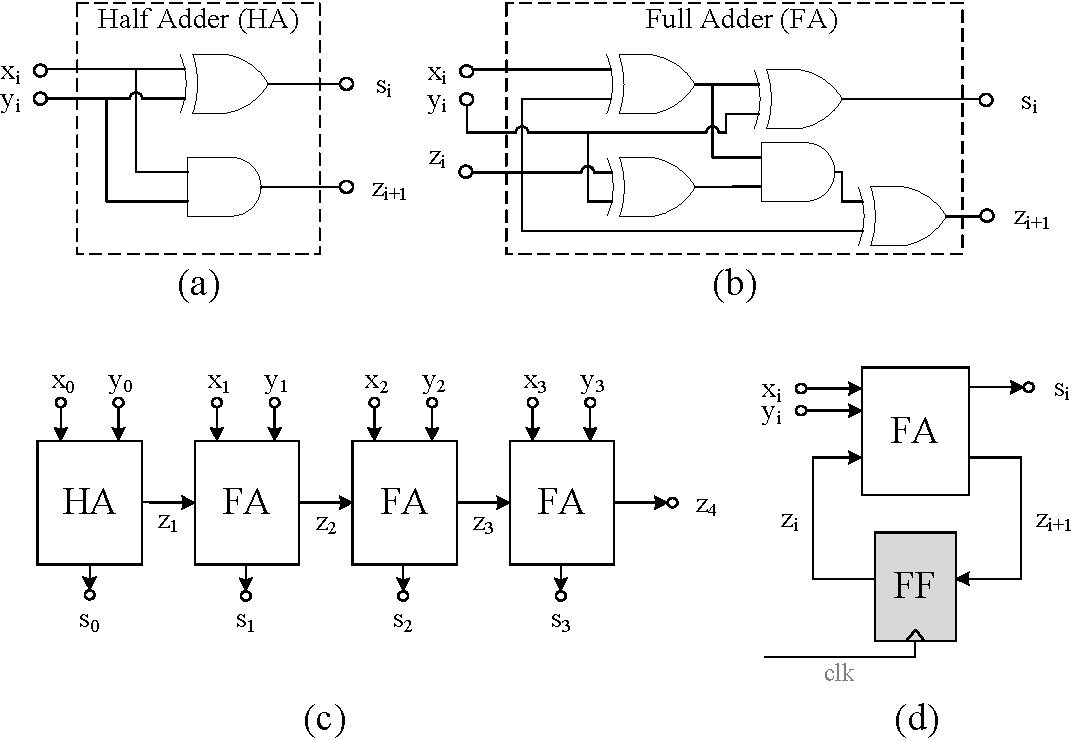
\includegraphics[width=0.85\textwidth]{adder-crop.pdf}
    \caption{Combinational and sequential design of a 4-bit Adder.
  (a) \acrshort{ha} circuit.
  (b) \acrshort{fa} circuit.
  (c) Combinational 4-bit Adder using 1 \acrshort{ha} and 3 \acrshort{fa}s.
  (d) Sequential 4-bit Adder using one \acrshort{fa}.}\label{fig:combSeq}
\end{figure}

\fig{fig:combSeq} demonstrates an example of a combinational and a sequential implementation for a 4-bit Adder function with inputs $x = \overline{x_3x_2x_1x_0}$ and $y = \overline{y_3y_2y_1y_0}$, producing sum $s = \overline{s_3s_2s_1s_0} = f(x, y) = x + y$.
\fig{fig:combSeq}a and \ref{fig:combSeq}b show the internal combinational circuit of a half Adder (\acrshort{ha}) and a full Adder (\acrshort{fa}) respectively.
In \fig{fig:combSeq}c a combinational Adder is built by cascading 3 \acrshort{fa}s and one \acrshort{ha}.
\fig{fig:combSeq}d represents a sequential implementation of a 4-bit Adder which uses one \acrshort{fa} and a one bit \acrshort{ff} to save the carry bit from the previous cycle.
The circuit should be evaluated for 4 cycles.
At the first cycle the carry bit is $z_0=0$.
Note that, in the combinational circuit we use three \acrshort{fa}s and one \acrshort{ha} whereas in the sequential circuit, we have to use one \acrshort{fa} for 4 sequential cycles.
This asymmetry in the loop of Addition function introduces a small \emph{overhead} in \acrshort{gc} computation and communication time as an \acrshort{ha} circuit has fewer gates compared to a \acrshort{fa} circuit.
We will discuss the overhead of garbling sequential circuits and its sources in more detail in \sect{sec:seq-overhead}.

However, the total number of gates for representing the function is reduced approximately by a factor of 4 when using a sequential circuit (one \acrshort{fa} for sequential compared with three \acrshort{fa} and one \acrshort{ha} for combinational).
This helps to limit the memory footprint for garbling and evaluation required for storing circuit description and wire labels ($k$-bit per wire, see \sect{ssec:prelim-gc}).
In a sequential circuit, the number of labels that need to be stored in memory at any moment is proportional to the number of gates in the circuit.
The wire labels are simply over-written at each sequential cycle.
Only labels corresponding to \acrshort{ff}s are kept for the next cycle.

Nearly all commercial circuits used in digital hardware are designed in sequential format.
There are multiple reasons for preferring sequential circuit description over combinational including the reduction in complexity, area, power, and cost, as well as natural mapping of finite state machine control functions into a sequential format.
Some of these reasons also provide a rationale for sequential description of a function in \acrshort{gc}, including: (i) reduction in size and memory footprint that is achieved by introducing the state elements and feedback loop from output to input; (ii) removing the need to perform costly compile-time/runtime loop unrolling by embracing loops within the sequential feedback loop; (iii) providing a new degree of freedom for folding by the placement of memory elements in the long combinational paths--the placement can be done in accordance with the user's objective; (iv) solving the limitation of synthesis techniques and tools for large function (see /sec{sect:syn-limit}) by describing circuits in compact sequential format.

\begin{figure}
  \centering
  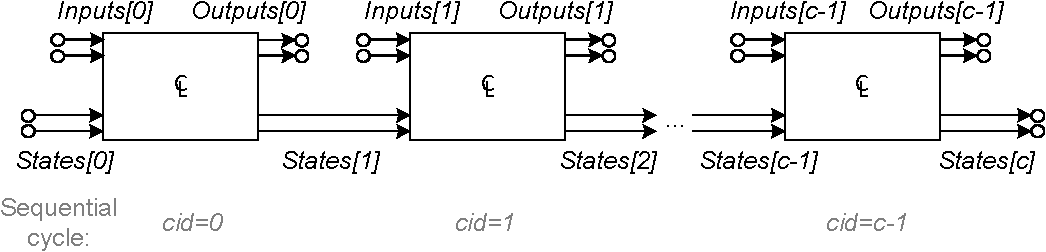
\includegraphics[width=0.9\textwidth]{sequential-open-crop.pdf}
  \caption{Functionally equivalent unrolled sequential circuit corresponding to \fig{fig:sequential}.}
  \label{fig:open-sequential}
\end{figure}

During the evaluation of a sequential circuit, the combinational block is evaluated $cc$ times where $cc$ is the number of sequential cycles that the circuit operates.
We can visualize this process as the unrolled combinational representation of the sequential circuit as shown in \fig{fig:open-sequential}.
$cc$ also shows the folding factor of the sequential circuit ($cc=1$ means the circuit is combinational).
The inputs/outputs of the unrolled circuit are the inputs/outputs of the combinational block in all the cycles.
The present states at each cycle $\textrm{cid}$, where $0 \le \textrm{cid} < cc$, are equal to the next states at the previous cycle ($\textrm{cid}-1$).
The present states at $\textrm{cid}=0$ are equal to the input initial value.

In digital hardware, at edge of a cycle, the value of D of an \acrshort{ff} is latched and then transfered to the Q in the next sequential cycle.
In garbling/evaluating of a sequential circuit, an \acrshort{ff} operates as a simple wire connection between the the unrolled combinational circuit in two consecutive cycles.
Thus, it can be dealt with latching the labels from the flip-Flop input D in $\textrm{cid}$ to output Q in $\textrm{cid}+1$.
Signal clk and rst of \acrshort{ff} can be ignored in sequential \acrshort{gc}.

Garbling/evaluation of the sequential circuit is equivalent of garbling its gates for $cc$ times.
To make sure that the security and correctness of the \acrshort{gc} protocol still holds for the sequential circuits, we use combination of cycle index and gate identifier for the the encryption tweak $T$ (see \sect{sssec:prelim-aes}).
This way a unique tweak is assigned for the same gates in different cycles makes it same as garbling a unrolled combinational circuit.

In \appx{chap:engine}, we discuss our implementation of the \acrshort{gc} protocol for sequential circuits in \gls{tinygarble} \acrshort{gc} engine.
We also explain in more detail about how the encryption tweak is set and how it affects the security and correctness of the \acrshort{gc} protocol.

\section{Synthesis Sequential Circuit}\label{sec:seq-syn}
Fortunately, extending \gls{tinygarble} \acrshort{gc} synthesis to support sequential circuits is straightforward since the synthesis tools are designed to work them in the first place.
We add memory element of sequential circuits into the technology library of \gls{tinygarble} (see \sect{sec:syn-techlib}).
These elements can be implemented as \acrshort{ff}s which are connected to a clock signal.
Although in conventional \acrshort{asic} design \acrshort{ff}s are typically as costly as four NAND gates, as seen above in our \acrshort{gc} application, \acrshort{ff}s do not have any impact on the garbling/evaluation process as they require no cryptographic operations.
Therefore, we set the area of \acrshort{ff}s to 0 to show its lack of impact on computation and communication time of garbling/evaluation.
Moreover, we modify our \acrshort{ff}s such that they can accept an initial value.
This helps us remove extra \acrshort{mux}s in standard \acrshort{ff} design for initialization.

Describing functions using sequential circuits helps to overcome the scalability limitations of synthesis tool.
Sequential circuits are radically smaller than combinational ones with the same functionality.
This property allows synthesis tools to not only generates the circuit with less recourses, but to find a more optimized circuit.
Moreover, the compatibility of our sequential descriptions with standard synthesis tools simplifies the workflow of circuit generation for \acrshort{sfe} applications.

\section{Overhead of Sequential Circuit}\label{sec:seq-overhead}
In sequential circuit, the function is divided into smaller steps such that one step is computed at each cycle.
If a function can be divided into identical steps, only one step is implemented in the sequential circuit.
Evaluating the sequential circuit for multiple cycles ensures that the function is computed completely.
However, many functions does not have such symmetrical structure and cannot be divided perfectly into identical steps.
The sequential circuit of such a function includes different sub-circuits that each corresponds to one of the steps in the function.

\fig{fig:seq-overhead-comb} shows an example of such function that is represented as a combinational circuit.
The computation in the function can be divided into 6 non-identical steps.
The computation in the first and last steps are different from the rest.
U1 sub-circuit represents the computation in the first step, U2 the middle four steps, and U3 the last step.
\fig{fig:seq-overhead-seq} illustrates the sequential circuit representation of the example function.
A \acrshort{mux} selects the output of the sub-circuits according to the cycle id (cid).
In the digital circuit design, \acrshort{mux} and similar components that control the flow of data is called control path.
If cid is 0, U1 is selected, if it is 5, U3 is selected, otherwise U2 is selected.
The unselected sub-circuits remain idle in that cycle, since its output is not used.
At each cycle, the output of the selected sub-circuit is stored in the \acrshort{ff} to be used in the next cycles.

\begin{figure}
    \centering
    \begin{subfigure}[t]{0.7\textwidth}
        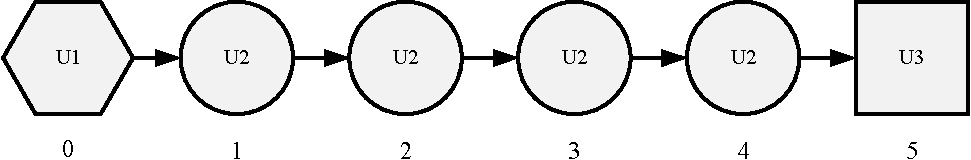
\includegraphics[width=\textwidth]{seq-overhead-comb-crop.pdf}
        \caption{Combination Circuit.}\label{fig:seq-overhead-comb}
    \end{subfigure}
    \begin{subfigure}[t]{0.6\textwidth}
        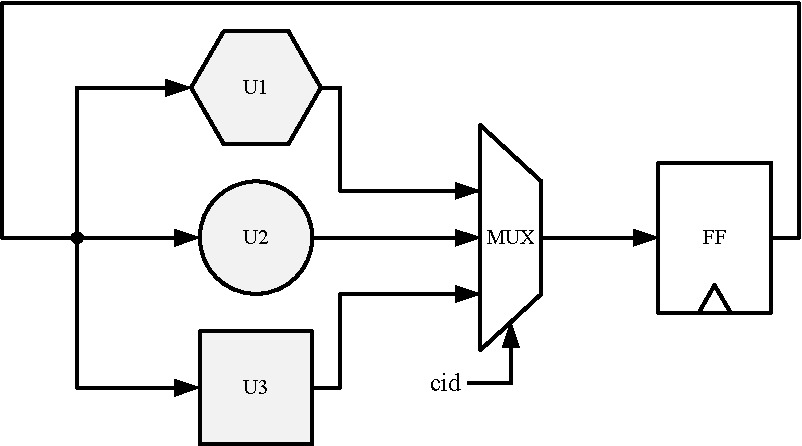
\includegraphics[width=\textwidth]{seq-overhead-seq-crop.pdf}
        \caption{Sequential Circuit.}\label{fig:seq-overhead-seq}
    \end{subfigure}\\
    \caption{The combinational and sequential representations of a function with an asymmetric structure.
    The sequential implementation has to be evaluated for 6 cycles and eventually needs more gates to be garbled/evaluated compared to the combinational one.}\label{fig:fig:seq-overhead-comb}
\end{figure}

The number of gates that has to garbled/evaluated in the combinational circuit is $C_{U1}+4*C_{U2}+C_{U3}$, where $C_{Ui}$ is the number of gates in $Ui$ sub-circuit.
Since the sequential circuit has to be garbled/evaluated for $cc=6$ times, the total gates for sequential circuit is $6*(C_{U1}+C_{U2}+C_{U3}+C_{\acrshort{mux}})$, where $C_{\acrshort{mux}}$ is number of non-XOR in the \acrshort{mux}.
The difference between the cost of the combinational and the sequential circuits is $5*C_{U1}+2*C_{U1}+5*C_{U3}+6*C_{\acrshort{mux}})$.
We call this difference the sequential \textit{overhead} for garbling an asymmetrical function.

The overhead is caused by treating cid as a secret value in the \acrshort{gc} protocol while both parties known its value at all cycles.
In the next chapter, we will discuss how to reduce this overhead using a novel algorithm on top of sequential \acrshort{gc} protocol.
The algorithm skips unnecessary garbling/evaluation of idle sub-circuits and allows local computation of the gates in the control path.
